% !TeX root = ..\main.tex
%%%%%%%%%%%%%%%%%%%%%%%%%  
\section{Cấu trúc mã nguồn}
\subsection{Cấu trúc front-end}
\begin{figure}[!htp]
    \begin{center}
        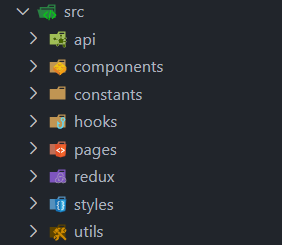
\includegraphics[width=7cm]{img/file-structure/front-end.png}
    \end{center}
    \caption{Cấu trúc mã nguồn front-end}
\end{figure}

Hệ thống thư mục bao gồm:
\begin{itemize}
    \item api:
    \item component:
    \item constants:
    \item hooks:
    \item pages:
    \item redux:
    \item style:
    \item util:
\end{itemize}


\subsection{Cấu trúc back-end}
\begin{figure}[!htp]
    \begin{center}
        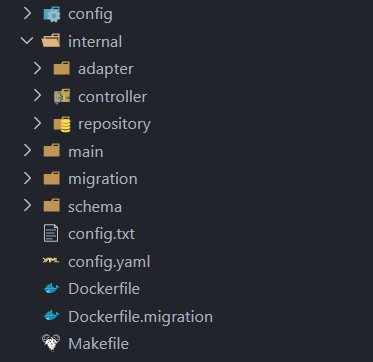
\includegraphics[width=7cm]{img/file-structure/back-end.png}
    \end{center}
    \caption{Cấu trúc mã nguồn back-end}
\end{figure}

Hệ thống thư mục bao gồm:
\begin{itemize}
    \item config:
    \item internal: Bao gồm các thư mục
          \begin{itemize}
              \item adapter:
          \end{itemize}
    \item main:
    \item migration:
    \item schema:
\end{itemize}

\subsection{Cấu trúc BPEL}

\begin{figure}[!htp]
    \begin{center}
        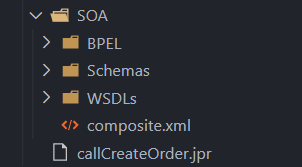
\includegraphics[width=6cm]{img/file-structure/bpel.png}
    \end{center}
    \caption{Cấu trúc mã nguồn bpel}
\end{figure}

\begin{itemize}
    \item BPEL:
    \item Schemas:
    \item WSDLs:
    \item file .jpr:
\end{itemize}